

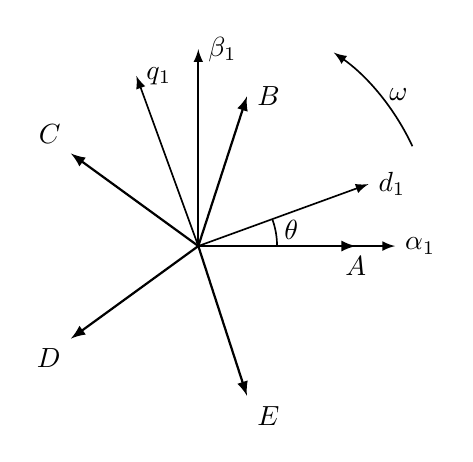
\begin{tikzpicture}[>=latex, line width=0.6pt]

\begin{scope}[shift={(0,0)}]
% Osy alpha a beta
    \draw[->] (0,0) -- (2.5,0) node[right] {$\alpha_1$};
    \draw[->] (0,0) -- (0,2.5) node[right] {$\beta_1$};
    
    % Vektory fází A-E (délka 2.0)
    \draw[->, thick] (0,0) -- (0:2) node[below] {$A$};
    \draw[->, thick] (0,0) -- (72:2) node[right] {$B$};
    \draw[->, thick] (0,0) -- (144:2) node[above left] {$C$};
    \draw[->, thick] (0,0) -- (216:2) node[below left] {$D$};
    \draw[->, thick] (0,0) -- (288:2) node[below right] {$E$};
    
    % d-q soustava (délka 2.3)
    \def\thetaang{20}
    \draw[->] (0,0) -- (\thetaang:2.3) node[right] {$d_1$};
    \draw[->] (0,0) -- (\thetaang+90:2.3) node[right] {$q_1$};
    
    % Úhel theta
    \draw (\thetaang:1.0) arc (\thetaang:0:1.0);
    \node at (10:1.2) {$\theta$};
    
    % ŠIPKA OMEGA - nyní na poloměru 3.0 (velmi daleko)
    \draw[->, bend left=30] (25:3.0) arc (25:55:3.0) node[midway, right] {$\omega$};
    
\end{scope}
\end{tikzpicture}